\subsection{Summary of Findings}
\label{sec:expt_summary}

The previous sections described the basic framework for \SeeDB and the suite of sharing and pruning optimizations we developed for \SeeDB.
% two suits of optimizations to efficiently process, we developed a basic framework and sets of pruning an sharing optimizations for \SeeDB.
Figure \ref{} shows a summary of \SeeDB performance for the four real datasets from Table \ref{tab:datasets}, namely BANK, DIAB, AIR and AIR10. 
For each dataset, we show the latencies obtained by the basic \SeeDB framework (NO\_OPT), by our sharing optimizations (SHARING), and by the combination of our sharing and pruning optimizations (SH\_PR\_EARLY for early stopping and SH\_PR\_FULL for full processing).
(This figure shows results for ROW. Results for COL are discussed further in Section \ref{}).
We find that:

\begin{figure}[h]
	\centering
	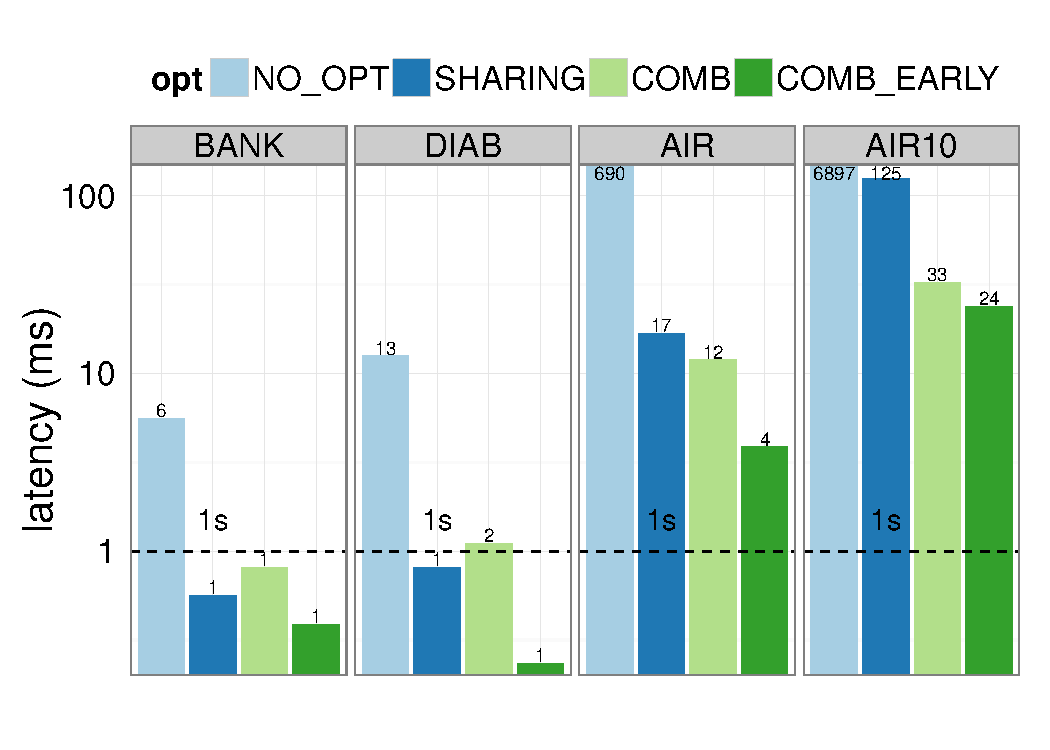
\includegraphics[width=8.4cm] {Images/all_opt_real_data_row.pdf}
	\caption{Performance gains of all optimizations in ROW}
	\label{fig:share_prune_row}
	\vspace{-15pt}
\end{figure}

\begin{denselist} 
\item The combination of our sharing and pruning optimizations provide a speedup of upto 40X (SH\_PR\_FULL) -- 100X (SH\_PR\_EARLY) for ROW (shown above) and 10 -- 20X for COL.
This reduces latencies for small datasets like DIAB from 12s to 200ms, and from >1 hr to <30s for large datasets like AIR10.
\item The sharing optimizations from Section \ref{} produce performance gains of upto 40X for ROW and 10X for COL. This enables \SeeDB to process small and moderate sized datasets (1M rows, 100 views) in interactive time scales, i.e. within a few seconds.
\item Pruning optimizations from Section \ref{} provide additional gains of 2X -- 5X by rapidly pruning low-utility views. Early result return can provide particularly significant gains and enable real-time response for large datasets. We also find that quality of results is not adversely affected by pruning, the visualizations returned by \SeeDB have utility very close to the actual top-$k$ utilities.
\item In general, COL stores are better suited to the \SeeDB workload and outperform ROW stores. The reason is that the data layout for COL enables only those attributes involved in the view to be read and processed. 
\item Finally, we observe that while our techniques show performance gains across the board, theya are particularly useful for large datasets with hundreds of views. For instance, one of the biggest performance gains we observe (50X) is for AIR10 (60M rows, 108 views).
\end{denselist}

In the next sections, we discuss the performance of individual optimizations and how they relate to the overall performance gain.



